% generated by Plantuml 1.2018.13      
\definecolor{plantucolor0000}{RGB}{0,0,0}
\definecolor{plantucolor0001}{RGB}{254,254,206}
\definecolor{plantucolor0002}{RGB}{168,0,54}
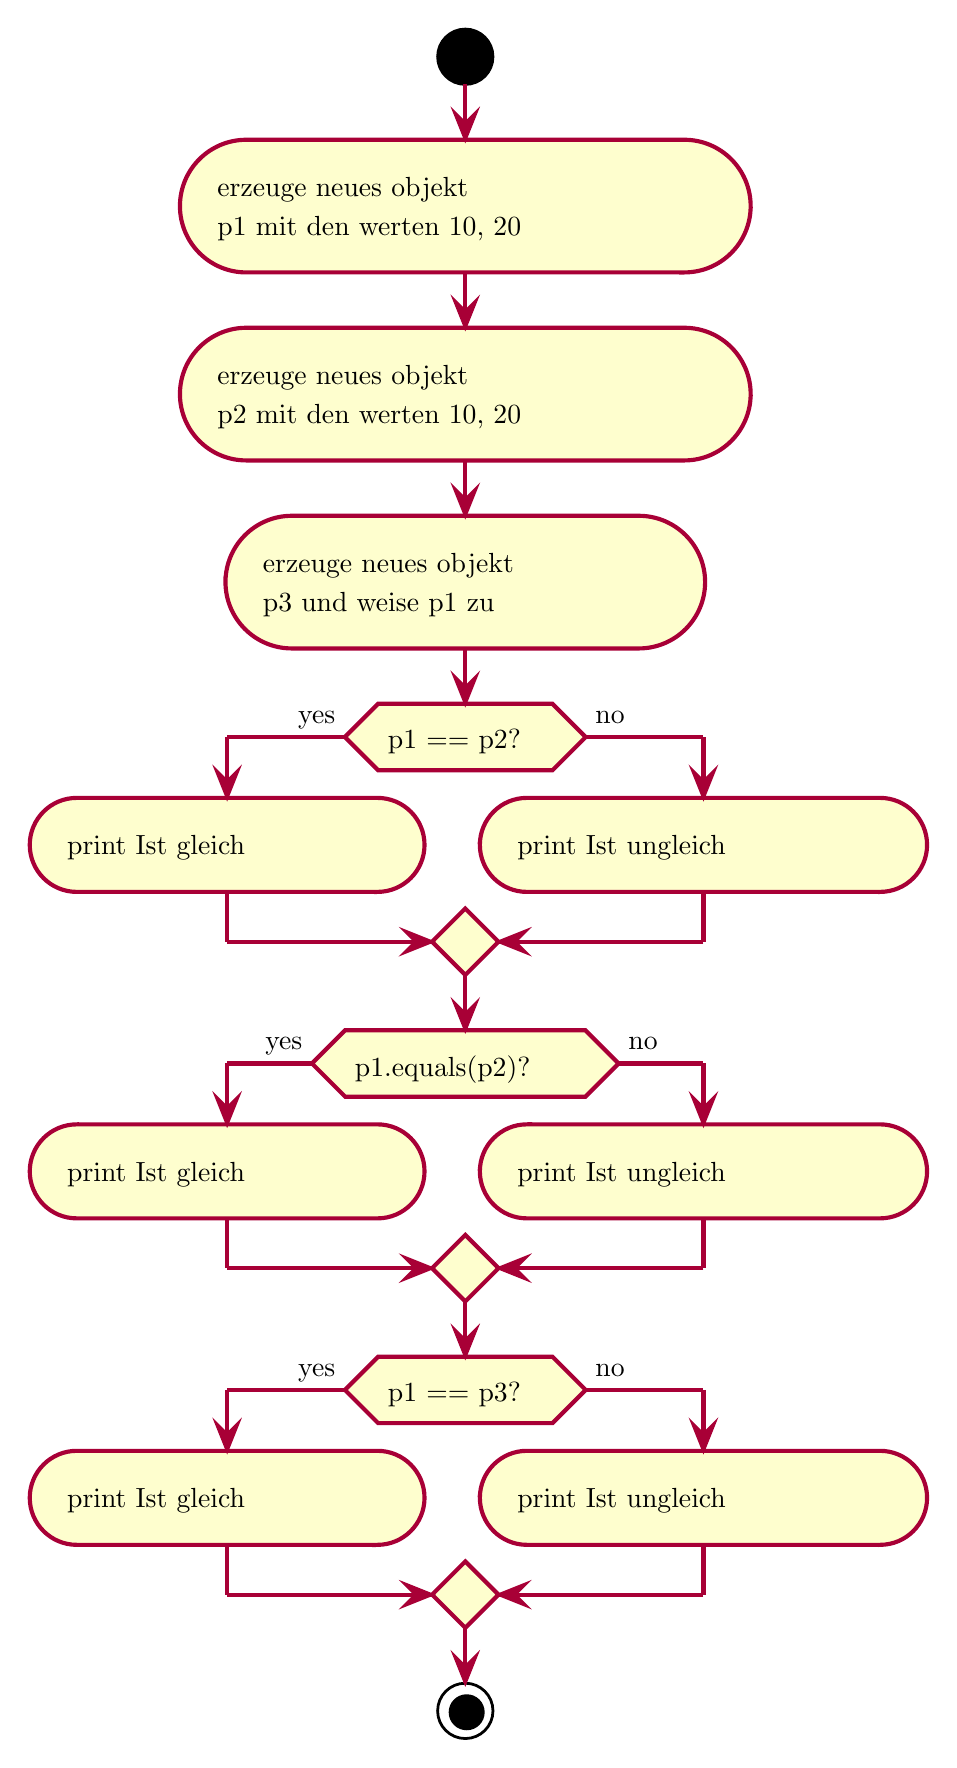
\begin{tikzpicture}[yscale=-1
,pstyle0/.style={fill=black,line width=1.0pt}
,pstyle1/.style={color=plantucolor0002,fill=plantucolor0001,line width=1.5pt}
,pstyle3/.style={color=plantucolor0002,line width=1.5pt}
,pstyle4/.style={color=plantucolor0002,fill=plantucolor0002,line width=1.0pt}
]
\draw[pstyle0] (167.3846pt,20pt) ellipse (10pt and 10pt);
\draw[pstyle1] (64.2739pt,73.9688pt) arc (180:270:23.9688pt) -- (88.2427pt,50pt) -- (246.5266pt,50pt) arc (270:360:23.9688pt) -- (270.4953pt,73.9688pt) -- (270.4953pt,73.9688pt) arc (0:90:23.9688pt) -- (246.5266pt,97.9375pt) -- (88.2427pt,97.9375pt) arc (90:180:23.9688pt) -- (64.2739pt,73.9688pt) -- cycle;
\node at (74.2739pt,60pt)[below right,color=black]{erzeuge neues objekt};
\node at (74.2739pt,73.9688pt)[below right,color=black]{p1 mit den werten 10, 20};
\draw[pstyle1] (64.2739pt,141.9063pt) arc (180:270:23.9688pt) -- (88.2427pt,117.9375pt) -- (246.5266pt,117.9375pt) arc (270:360:23.9688pt) -- (270.4953pt,141.9063pt) -- (270.4953pt,141.9063pt) arc (0:90:23.9688pt) -- (246.5266pt,165.875pt) -- (88.2427pt,165.875pt) arc (90:180:23.9688pt) -- (64.2739pt,141.9063pt) -- cycle;
\node at (74.2739pt,127.9375pt)[below right,color=black]{erzeuge neues objekt};
\node at (74.2739pt,141.9063pt)[below right,color=black]{p2 mit den werten 10, 20};
\draw[pstyle1] (80.7301pt,209.8438pt) arc (180:270:23.9688pt) -- (104.6988pt,185.875pt) -- (230.0704pt,185.875pt) arc (270:360:23.9688pt) -- (254.0392pt,209.8438pt) -- (254.0392pt,209.8438pt) arc (0:90:23.9688pt) -- (230.0704pt,233.8125pt) -- (104.6988pt,233.8125pt) arc (90:180:23.9688pt) -- (80.7301pt,209.8438pt) -- cycle;
\node at (90.7301pt,195.875pt)[below right,color=black]{erzeuge neues objekt};
\node at (90.7301pt,209.8438pt)[below right,color=black]{p3 und weise p1 zu};
\draw[pstyle1] (135.8846pt,253.8125pt) -- (198.8846pt,253.8125pt) -- (210.8846pt,265.8125pt) -- (198.8846pt,277.8125pt) -- (135.8846pt,277.8125pt) -- (123.8846pt,265.8125pt) -- (135.8846pt,253.8125pt) -- cycle;
\node at (135.8846pt,259.4102pt)[below right,color=black]{p1 == p2?};
\node at (103.4846pt,253.0078pt)[below right,color=black]{yes};
\node at (210.8846pt,253.0078pt)[below right,color=black]{no};
\draw[pstyle1] (10pt,304.7969pt) arc (180:270:16.9844pt) -- (26.9844pt,287.8125pt) -- (135.6618pt,287.8125pt) arc (270:360:16.9844pt) -- (152.6462pt,304.7969pt) -- (152.6462pt,304.7969pt) arc (0:90:16.9844pt) -- (135.6618pt,321.7813pt) -- (26.9844pt,321.7813pt) arc (90:180:16.9844pt) -- (10pt,304.7969pt) -- cycle;
\node at (20pt,297.8125pt)[below right,color=black]{print \dq Ist gleich\dq};
\draw[pstyle1] (172.6462pt,304.7969pt) arc (180:270:16.9844pt) -- (189.6305pt,287.8125pt) -- (317.2618pt,287.8125pt) arc (270:360:16.9844pt) -- (334.2462pt,304.7969pt) -- (334.2462pt,304.7969pt) arc (0:90:16.9844pt) -- (317.2618pt,321.7813pt) -- (189.6305pt,321.7813pt) arc (90:180:16.9844pt) -- (172.6462pt,304.7969pt) -- cycle;
\node at (182.6462pt,297.8125pt)[below right,color=black]{print \dq Ist ungleich\dq };
\draw[pstyle1] (167.3846pt,327.7813pt) -- (179.3846pt,339.7813pt) -- (167.3846pt,351.7813pt) -- (155.3846pt,339.7813pt) -- (167.3846pt,327.7813pt) -- cycle;
\draw[pstyle1] (123.9698pt,371.7813pt) -- (210.7994pt,371.7813pt) -- (222.7994pt,383.7813pt) -- (210.7994pt,395.7813pt) -- (123.9698pt,395.7813pt) -- (111.9698pt,383.7813pt) -- (123.9698pt,371.7813pt) -- cycle;
\node at (123.9698pt,377.3789pt)[below right,color=black]{p1.equals(p2)?};
\node at (91.5698pt,370.9766pt)[below right,color=black]{yes};
\node at (222.7994pt,370.9766pt)[below right,color=black]{no};
\draw[pstyle1] (10pt,422.7656pt) arc (180:270:16.9844pt) -- (26.9844pt,405.7813pt) -- (135.6618pt,405.7813pt) arc (270:360:16.9844pt) -- (152.6462pt,422.7656pt) -- (152.6462pt,422.7656pt) arc (0:90:16.9844pt) -- (135.6618pt,439.75pt) -- (26.9844pt,439.75pt) arc (90:180:16.9844pt) -- (10pt,422.7656pt) -- cycle;
\node at (20pt,415.7813pt)[below right,color=black]{print \dq Ist gleich\dq };
\draw[pstyle1] (172.6462pt,422.7656pt) arc (180:270:16.9844pt) -- (189.6305pt,405.7813pt) -- (317.2618pt,405.7813pt) arc (270:360:16.9844pt) -- (334.2462pt,422.7656pt) -- (334.2462pt,422.7656pt) arc (0:90:16.9844pt) -- (317.2618pt,439.75pt) -- (189.6305pt,439.75pt) arc (90:180:16.9844pt) -- (172.6462pt,422.7656pt) -- cycle;
\node at (182.6462pt,415.7813pt)[below right,color=black]{print \dq Ist ungleich\dq };
\draw[pstyle1] (167.3846pt,445.75pt) -- (179.3846pt,457.75pt) -- (167.3846pt,469.75pt) -- (155.3846pt,457.75pt) -- (167.3846pt,445.75pt) -- cycle;
\draw[pstyle1] (135.8846pt,489.75pt) -- (198.8846pt,489.75pt) -- (210.8846pt,501.75pt) -- (198.8846pt,513.75pt) -- (135.8846pt,513.75pt) -- (123.8846pt,501.75pt) -- (135.8846pt,489.75pt) -- cycle;
\node at (135.8846pt,495.3477pt)[below right,color=black]{p1 == p3?};
\node at (103.4846pt,488.9453pt)[below right,color=black]{yes};
\node at (210.8846pt,488.9453pt)[below right,color=black]{no};
\draw[pstyle1] (10pt,540.7344pt) arc (180:270:16.9844pt) -- (26.9844pt,523.75pt) -- (135.6618pt,523.75pt) arc (270:360:16.9844pt) -- (152.6462pt,540.7344pt) -- (152.6462pt,540.7344pt) arc (0:90:16.9844pt) -- (135.6618pt,557.7188pt) -- (26.9844pt,557.7188pt) arc (90:180:16.9844pt) -- (10pt,540.7344pt) -- cycle;
\node at (20pt,533.75pt)[below right,color=black]{print \dq Ist gleich\dq };
\draw[pstyle1] (172.6462pt,540.7344pt) arc (180:270:16.9844pt) -- (189.6305pt,523.75pt) -- (317.2618pt,523.75pt) arc (270:360:16.9844pt) -- (334.2462pt,540.7344pt) -- (334.2462pt,540.7344pt) arc (0:90:16.9844pt) -- (317.2618pt,557.7188pt) -- (189.6305pt,557.7188pt) arc (90:180:16.9844pt) -- (172.6462pt,540.7344pt) -- cycle;
\node at (182.6462pt,533.75pt)[below right,color=black]{print \dq Ist ungleich\dq };
\draw[pstyle1] (167.3846pt,563.7188pt) -- (179.3846pt,575.7188pt) -- (167.3846pt,587.7188pt) -- (155.3846pt,575.7188pt) -- (167.3846pt,563.7188pt) -- cycle;
\draw[color=black,line width=1.0pt] (167.3846pt,617.7188pt) ellipse (10pt and 10pt);
\draw[pstyle0] (167.8846pt,618.2188pt) ellipse (6pt and 6pt);
\draw[pstyle3] (167.3846pt,30pt) -- (167.3846pt,50pt);
\draw[pstyle4] (163.3846pt,40pt) -- (167.3846pt,50pt) -- (171.3846pt,40pt) -- (167.3846pt,44pt) -- cycle;
\draw[pstyle3] (167.3846pt,97.9375pt) -- (167.3846pt,117.9375pt);
\draw[pstyle4] (163.3846pt,107.9375pt) -- (167.3846pt,117.9375pt) -- (171.3846pt,107.9375pt) -- (167.3846pt,111.9375pt) -- cycle;
\draw[pstyle3] (167.3846pt,165.875pt) -- (167.3846pt,185.875pt);
\draw[pstyle4] (163.3846pt,175.875pt) -- (167.3846pt,185.875pt) -- (171.3846pt,175.875pt) -- (167.3846pt,179.875pt) -- cycle;
\draw[pstyle3] (123.8846pt,265.8125pt) -- (81.3231pt,265.8125pt);
\draw[pstyle3] (81.3231pt,265.8125pt) -- (81.3231pt,287.8125pt);
\draw[pstyle4] (77.3231pt,277.8125pt) -- (81.3231pt,287.8125pt) -- (85.3231pt,277.8125pt) -- (81.3231pt,281.8125pt) -- cycle;
\draw[pstyle3] (210.8846pt,265.8125pt) -- (253.4462pt,265.8125pt);
\draw[pstyle3] (253.4462pt,265.8125pt) -- (253.4462pt,287.8125pt);
\draw[pstyle4] (249.4462pt,277.8125pt) -- (253.4462pt,287.8125pt) -- (257.4462pt,277.8125pt) -- (253.4462pt,281.8125pt) -- cycle;
\draw[pstyle3] (81.3231pt,321.7813pt) -- (81.3231pt,339.7813pt);
\draw[pstyle3] (81.3231pt,339.7813pt) -- (155.3846pt,339.7813pt);
\draw[pstyle4] (145.3846pt,335.7813pt) -- (155.3846pt,339.7813pt) -- (145.3846pt,343.7813pt) -- (149.3846pt,339.7813pt) -- cycle;
\draw[pstyle3] (253.4462pt,321.7813pt) -- (253.4462pt,339.7813pt);
\draw[pstyle3] (253.4462pt,339.7813pt) -- (179.3846pt,339.7813pt);
\draw[pstyle4] (189.3846pt,335.7813pt) -- (179.3846pt,339.7813pt) -- (189.3846pt,343.7813pt) -- (185.3846pt,339.7813pt) -- cycle;
\draw[pstyle3] (167.3846pt,233.8125pt) -- (167.3846pt,253.8125pt);
\draw[pstyle4] (163.3846pt,243.8125pt) -- (167.3846pt,253.8125pt) -- (171.3846pt,243.8125pt) -- (167.3846pt,247.8125pt) -- cycle;
\draw[pstyle3] (111.9698pt,383.7813pt) -- (81.3231pt,383.7813pt);
\draw[pstyle3] (81.3231pt,383.7813pt) -- (81.3231pt,405.7813pt);
\draw[pstyle4] (77.3231pt,395.7813pt) -- (81.3231pt,405.7813pt) -- (85.3231pt,395.7813pt) -- (81.3231pt,399.7813pt) -- cycle;
\draw[pstyle3] (222.7994pt,383.7813pt) -- (253.4462pt,383.7813pt);
\draw[pstyle3] (253.4462pt,383.7813pt) -- (253.4462pt,405.7813pt);
\draw[pstyle4] (249.4462pt,395.7813pt) -- (253.4462pt,405.7813pt) -- (257.4462pt,395.7813pt) -- (253.4462pt,399.7813pt) -- cycle;
\draw[pstyle3] (81.3231pt,439.75pt) -- (81.3231pt,457.75pt);
\draw[pstyle3] (81.3231pt,457.75pt) -- (155.3846pt,457.75pt);
\draw[pstyle4] (145.3846pt,453.75pt) -- (155.3846pt,457.75pt) -- (145.3846pt,461.75pt) -- (149.3846pt,457.75pt) -- cycle;
\draw[pstyle3] (253.4462pt,439.75pt) -- (253.4462pt,457.75pt);
\draw[pstyle3] (253.4462pt,457.75pt) -- (179.3846pt,457.75pt);
\draw[pstyle4] (189.3846pt,453.75pt) -- (179.3846pt,457.75pt) -- (189.3846pt,461.75pt) -- (185.3846pt,457.75pt) -- cycle;
\draw[pstyle3] (167.3846pt,351.7813pt) -- (167.3846pt,371.7813pt);
\draw[pstyle4] (163.3846pt,361.7813pt) -- (167.3846pt,371.7813pt) -- (171.3846pt,361.7813pt) -- (167.3846pt,365.7813pt) -- cycle;
\draw[pstyle3] (123.8846pt,501.75pt) -- (81.3231pt,501.75pt);
\draw[pstyle3] (81.3231pt,501.75pt) -- (81.3231pt,523.75pt);
\draw[pstyle4] (77.3231pt,513.75pt) -- (81.3231pt,523.75pt) -- (85.3231pt,513.75pt) -- (81.3231pt,517.75pt) -- cycle;
\draw[pstyle3] (210.8846pt,501.75pt) -- (253.4462pt,501.75pt);
\draw[pstyle3] (253.4462pt,501.75pt) -- (253.4462pt,523.75pt);
\draw[pstyle4] (249.4462pt,513.75pt) -- (253.4462pt,523.75pt) -- (257.4462pt,513.75pt) -- (253.4462pt,517.75pt) -- cycle;
\draw[pstyle3] (81.3231pt,557.7188pt) -- (81.3231pt,575.7188pt);
\draw[pstyle3] (81.3231pt,575.7188pt) -- (155.3846pt,575.7188pt);
\draw[pstyle4] (145.3846pt,571.7188pt) -- (155.3846pt,575.7188pt) -- (145.3846pt,579.7188pt) -- (149.3846pt,575.7188pt) -- cycle;
\draw[pstyle3] (253.4462pt,557.7188pt) -- (253.4462pt,575.7188pt);
\draw[pstyle3] (253.4462pt,575.7188pt) -- (179.3846pt,575.7188pt);
\draw[pstyle4] (189.3846pt,571.7188pt) -- (179.3846pt,575.7188pt) -- (189.3846pt,579.7188pt) -- (185.3846pt,575.7188pt) -- cycle;
\draw[pstyle3] (167.3846pt,469.75pt) -- (167.3846pt,489.75pt);
\draw[pstyle4] (163.3846pt,479.75pt) -- (167.3846pt,489.75pt) -- (171.3846pt,479.75pt) -- (167.3846pt,483.75pt) -- cycle;
\draw[pstyle3] (167.3846pt,587.7188pt) -- (167.3846pt,607.7188pt);
\draw[pstyle4] (163.3846pt,597.7188pt) -- (167.3846pt,607.7188pt) -- (171.3846pt,597.7188pt) -- (167.3846pt,601.7188pt) -- cycle;
\end{tikzpicture}
